% Created by tikzDevice version 0.12.6 on 2025-02-12 13:10:41
% !TEX encoding = UTF-8 Unicode
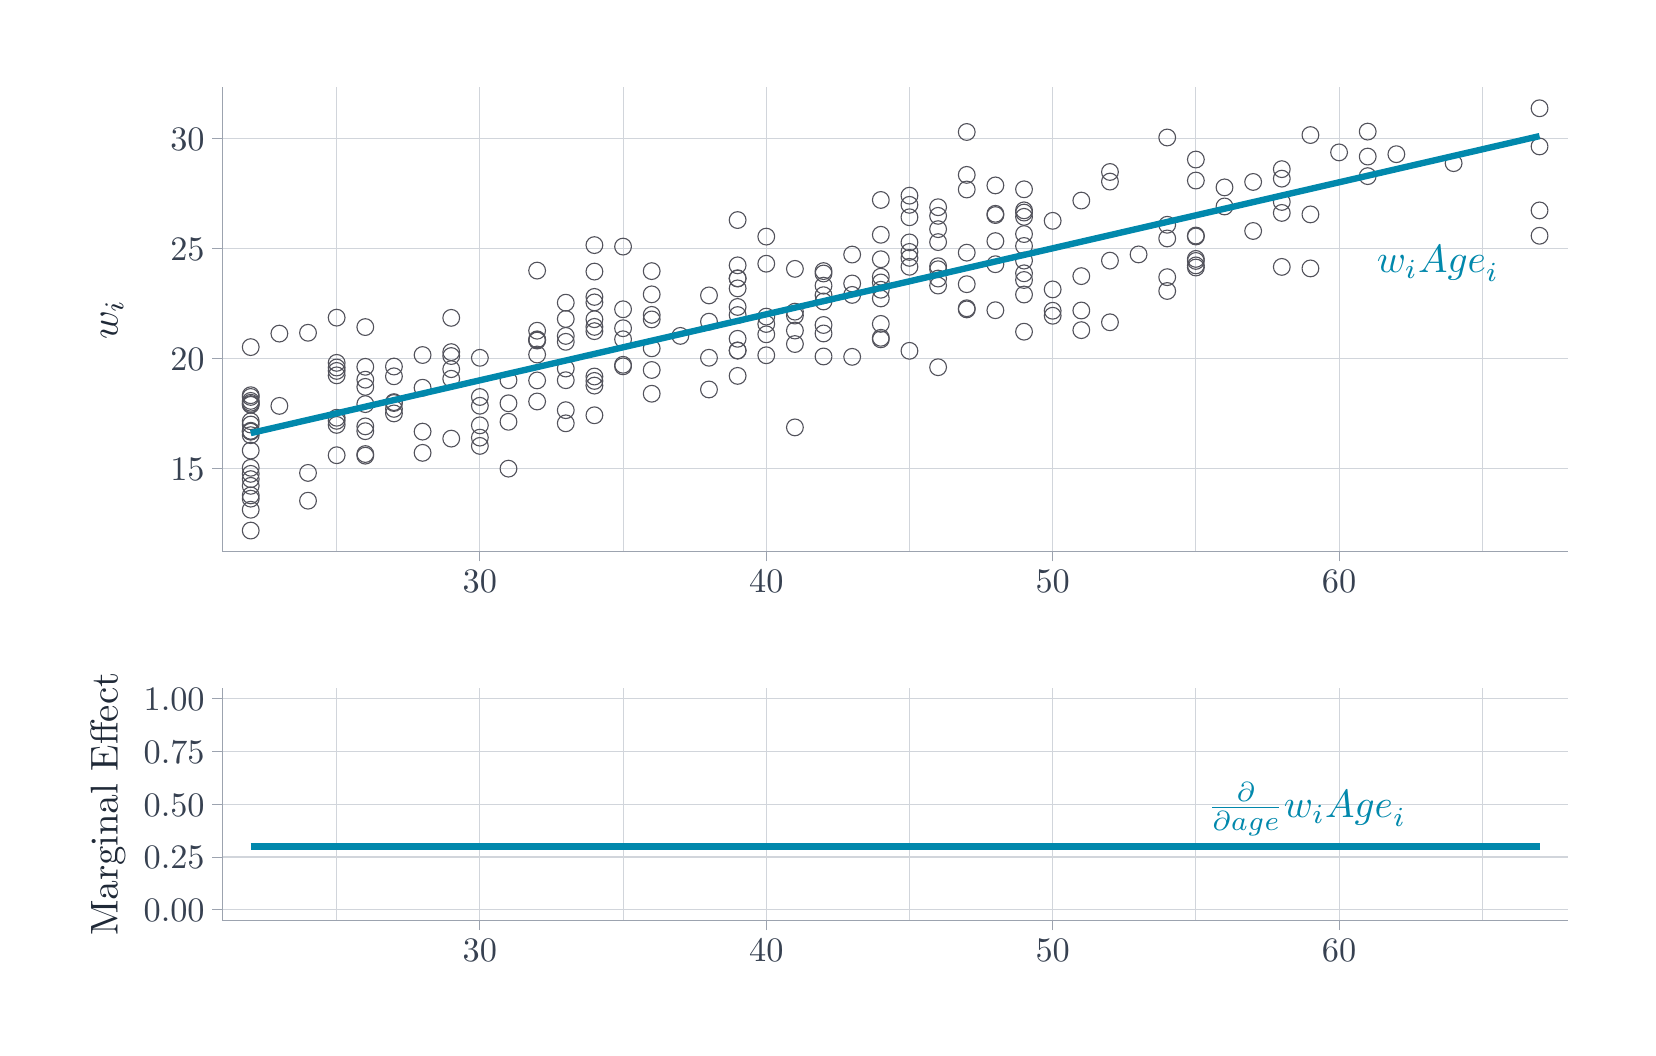
\begin{tikzpicture}[x=1pt,y=1pt]
\definecolor{fillColor}{RGB}{255,255,255}
\path[use as bounding box,fill=fillColor] (0,0) rectangle (578.16,361.35);
\begin{scope}
\path[clip] (  0.00,  0.00) rectangle (578.16,361.35);
\definecolor{drawColor}{RGB}{255,255,255}

\path[draw=drawColor,line width= 0.6pt,line join=round,line cap=round,fill=fillColor] (  0.00, -0.00) rectangle (578.16,361.35);
\end{scope}
\begin{scope}
\path[clip] (  5.50,138.71) rectangle (572.66,355.85);
\definecolor{drawColor}{RGB}{255,255,255}
\definecolor{fillColor}{RGB}{255,255,255}

\path[draw=drawColor,line width= 0.7pt,line join=round,line cap=round,fill=fillColor] (  5.50,138.71) rectangle (572.66,355.85);
\end{scope}
\begin{scope}
\path[clip] (  5.50,  5.50) rectangle (572.66,138.71);
\definecolor{drawColor}{RGB}{255,255,255}
\definecolor{fillColor}{RGB}{255,255,255}

\path[draw=drawColor,line width= 0.7pt,line join=round,line cap=round,fill=fillColor] (  5.50,  5.50) rectangle (572.66,138.71);
\end{scope}
\begin{scope}
\path[clip] ( 70.25,172.00) rectangle (556.66,339.85);
\definecolor{drawColor}{RGB}{255,255,255}
\definecolor{fillColor}{RGB}{255,255,255}

\path[draw=drawColor,line width= 0.7pt,line join=round,line cap=round,fill=fillColor] ( 70.25,172.00) rectangle (556.66,339.85);
\definecolor{drawColor}{RGB}{209,213,219}

\path[draw=drawColor,line width= 0.4pt,line join=round] (111.65,172.00) --
	(111.65,339.85);

\path[draw=drawColor,line width= 0.4pt,line join=round] (215.14,172.00) --
	(215.14,339.85);

\path[draw=drawColor,line width= 0.4pt,line join=round] (318.63,172.00) --
	(318.63,339.85);

\path[draw=drawColor,line width= 0.4pt,line join=round] (422.12,172.00) --
	(422.12,339.85);

\path[draw=drawColor,line width= 0.4pt,line join=round] (525.61,172.00) --
	(525.61,339.85);

\path[draw=drawColor,line width= 0.4pt,line join=round] ( 70.25,202.13) --
	(556.66,202.13);

\path[draw=drawColor,line width= 0.4pt,line join=round] ( 70.25,241.87) --
	(556.66,241.87);

\path[draw=drawColor,line width= 0.4pt,line join=round] ( 70.25,281.62) --
	(556.66,281.62);

\path[draw=drawColor,line width= 0.4pt,line join=round] ( 70.25,321.36) --
	(556.66,321.36);

\path[draw=drawColor,line width= 0.4pt,line join=round] (163.40,172.00) --
	(163.40,339.85);

\path[draw=drawColor,line width= 0.4pt,line join=round] (266.89,172.00) --
	(266.89,339.85);

\path[draw=drawColor,line width= 0.4pt,line join=round] (370.38,172.00) --
	(370.38,339.85);

\path[draw=drawColor,line width= 0.4pt,line join=round] (473.87,172.00) --
	(473.87,339.85);
\definecolor{drawColor}{RGB}{82,82,91}

\path[draw=drawColor,line width= 0.4pt,line join=round,line cap=round] (173.74,233.95) circle (  3.03);

\path[draw=drawColor,line width= 0.4pt,line join=round,line cap=round] ( 80.60,217.94) circle (  3.03);

\path[draw=drawColor,line width= 0.4pt,line join=round,line cap=round] ( 80.60,195.79) circle (  3.03);

\path[draw=drawColor,line width= 0.4pt,line join=round,line cap=round] (173.74,202.00) circle (  3.03);

\path[draw=drawColor,line width= 0.4pt,line join=round,line cap=round] (287.58,250.85) circle (  3.03);

\path[draw=drawColor,line width= 0.4pt,line join=round,line cap=round] (422.12,274.68) circle (  3.03);

\path[draw=drawColor,line width= 0.4pt,line join=round,line cap=round] (194.44,233.96) circle (  3.03);

\path[draw=drawColor,line width= 0.4pt,line join=round,line cap=round] (101.30,190.42) circle (  3.03);

\path[draw=drawColor,line width= 0.4pt,line join=round,line cap=round] (163.40,242.05) circle (  3.03);

\path[draw=drawColor,line width= 0.4pt,line join=round,line cap=round] (204.79,282.78) circle (  3.03);

\path[draw=drawColor,line width= 0.4pt,line join=round,line cap=round] (328.98,288.54) circle (  3.03);

\path[draw=drawColor,line width= 0.4pt,line join=round,line cap=round] (204.79,262.07) circle (  3.03);

\path[draw=drawColor,line width= 0.4pt,line join=round,line cap=round] (422.12,277.06) circle (  3.03);

\path[draw=drawColor,line width= 0.4pt,line join=round,line cap=round] (122.00,231.55) circle (  3.03);

\path[draw=drawColor,line width= 0.4pt,line join=round,line cap=round] (225.49,229.07) circle (  3.03);

\path[draw=drawColor,line width= 0.4pt,line join=round,line cap=round] (546.31,332.22) circle (  3.03);

\path[draw=drawColor,line width= 0.4pt,line join=round,line cap=round] (287.58,242.53) circle (  3.03);

\path[draw=drawColor,line width= 0.4pt,line join=round,line cap=round] (391.08,254.89) circle (  3.03);

\path[draw=drawColor,line width= 0.4pt,line join=round,line cap=round] (163.40,217.65) circle (  3.03);

\path[draw=drawColor,line width= 0.4pt,line join=round,line cap=round] (484.22,323.79) circle (  3.03);

\path[draw=drawColor,line width= 0.4pt,line join=round,line cap=round] (153.05,237.95) circle (  3.03);

\path[draw=drawColor,line width= 0.4pt,line join=round,line cap=round] (287.58,272.52) circle (  3.03);

\path[draw=drawColor,line width= 0.4pt,line join=round,line cap=round] (142.70,243.06) circle (  3.03);

\path[draw=drawColor,line width= 0.4pt,line join=round,line cap=round] (308.28,248.73) circle (  3.03);

\path[draw=drawColor,line width= 0.4pt,line join=round,line cap=round] ( 80.60,208.54) circle (  3.03);

\path[draw=drawColor,line width= 0.4pt,line join=round,line cap=round] (277.24,257.32) circle (  3.03);

\path[draw=drawColor,line width= 0.4pt,line join=round,line cap=round] (194.44,256.08) circle (  3.03);

\path[draw=drawColor,line width= 0.4pt,line join=round,line cap=round] (308.28,299.09) circle (  3.03);

\path[draw=drawColor,line width= 0.4pt,line join=round,line cap=round] (204.79,273.21) circle (  3.03);

\path[draw=drawColor,line width= 0.4pt,line join=round,line cap=round] ( 80.60,245.92) circle (  3.03);

\path[draw=drawColor,line width= 0.4pt,line join=round,line cap=round] (360.03,282.47) circle (  3.03);

\path[draw=drawColor,line width= 0.4pt,line join=round,line cap=round] ( 80.60,215.68) circle (  3.03);

\path[draw=drawColor,line width= 0.4pt,line join=round,line cap=round] (308.28,277.67) circle (  3.03);

\path[draw=drawColor,line width= 0.4pt,line join=round,line cap=round] (370.38,259.06) circle (  3.03);

\path[draw=drawColor,line width= 0.4pt,line join=round,line cap=round] (349.68,304.35) circle (  3.03);

\path[draw=drawColor,line width= 0.4pt,line join=round,line cap=round] (349.68,294.09) circle (  3.03);

\path[draw=drawColor,line width= 0.4pt,line join=round,line cap=round] (297.93,279.36) circle (  3.03);

\path[draw=drawColor,line width= 0.4pt,line join=round,line cap=round] (401.42,279.41) circle (  3.03);

\path[draw=drawColor,line width= 0.4pt,line join=round,line cap=round] ( 80.60,228.54) circle (  3.03);

\path[draw=drawColor,line width= 0.4pt,line join=round,line cap=round] ( 80.60,192.34) circle (  3.03);

\path[draw=drawColor,line width= 0.4pt,line join=round,line cap=round] (308.28,263.50) circle (  3.03);

\path[draw=drawColor,line width= 0.4pt,line join=round,line cap=round] (422.12,285.89) circle (  3.03);

\path[draw=drawColor,line width= 0.4pt,line join=round,line cap=round] (204.79,221.29) circle (  3.03);

\path[draw=drawColor,line width= 0.4pt,line join=round,line cap=round] (153.05,244.11) circle (  3.03);

\path[draw=drawColor,line width= 0.4pt,line join=round,line cap=round] (453.17,306.79) circle (  3.03);

\path[draw=drawColor,line width= 0.4pt,line join=round,line cap=round] (111.65,206.85) circle (  3.03);

\path[draw=drawColor,line width= 0.4pt,line join=round,line cap=round] (287.58,268.12) circle (  3.03);

\path[draw=drawColor,line width= 0.4pt,line join=round,line cap=round] (546.31,318.43) circle (  3.03);

\path[draw=drawColor,line width= 0.4pt,line join=round,line cap=round] (101.30,200.46) circle (  3.03);

\path[draw=drawColor,line width= 0.4pt,line join=round,line cap=round] (246.19,255.11) circle (  3.03);

\path[draw=drawColor,line width= 0.4pt,line join=round,line cap=round] (422.12,277.79) circle (  3.03);

\path[draw=drawColor,line width= 0.4pt,line join=round,line cap=round] (442.82,287.88) circle (  3.03);

\path[draw=drawColor,line width= 0.4pt,line join=round,line cap=round] (287.58,264.68) circle (  3.03);

\path[draw=drawColor,line width= 0.4pt,line join=round,line cap=round] (256.54,275.47) circle (  3.03);

\path[draw=drawColor,line width= 0.4pt,line join=round,line cap=round] (453.17,274.90) circle (  3.03);

\path[draw=drawColor,line width= 0.4pt,line join=round,line cap=round] (266.89,285.85) circle (  3.03);

\path[draw=drawColor,line width= 0.4pt,line join=round,line cap=round] (173.74,225.62) circle (  3.03);

\path[draw=drawColor,line width= 0.4pt,line join=round,line cap=round] (256.54,270.79) circle (  3.03);

\path[draw=drawColor,line width= 0.4pt,line join=round,line cap=round] (277.24,216.91) circle (  3.03);

\path[draw=drawColor,line width= 0.4pt,line join=round,line cap=round] (194.44,218.38) circle (  3.03);

\path[draw=drawColor,line width= 0.4pt,line join=round,line cap=round] (225.49,257.57) circle (  3.03);

\path[draw=drawColor,line width= 0.4pt,line join=round,line cap=round] (266.89,250.54) circle (  3.03);

\path[draw=drawColor,line width= 0.4pt,line join=round,line cap=round] (328.98,283.87) circle (  3.03);

\path[draw=drawColor,line width= 0.4pt,line join=round,line cap=round] (111.65,235.72) circle (  3.03);

\path[draw=drawColor,line width= 0.4pt,line join=round,line cap=round] (494.57,315.63) circle (  3.03);

\path[draw=drawColor,line width= 0.4pt,line join=round,line cap=round] (380.73,271.57) circle (  3.03);

\path[draw=drawColor,line width= 0.4pt,line join=round,line cap=round] (463.52,322.55) circle (  3.03);

\path[draw=drawColor,line width= 0.4pt,line join=round,line cap=round] (111.65,238.55) circle (  3.03);

\path[draw=drawColor,line width= 0.4pt,line join=round,line cap=round] (132.35,225.72) circle (  3.03);

\path[draw=drawColor,line width= 0.4pt,line join=round,line cap=round] (122.00,225.32) circle (  3.03);

\path[draw=drawColor,line width= 0.4pt,line join=round,line cap=round] (422.12,286.24) circle (  3.03);

\path[draw=drawColor,line width= 0.4pt,line join=round,line cap=round] (422.12,313.70) circle (  3.03);

\path[draw=drawColor,line width= 0.4pt,line join=round,line cap=round] (122.00,253.16) circle (  3.03);

\path[draw=drawColor,line width= 0.4pt,line join=round,line cap=round] (277.24,247.03) circle (  3.03);

\path[draw=drawColor,line width= 0.4pt,line join=round,line cap=round] (142.70,207.71) circle (  3.03);

\path[draw=drawColor,line width= 0.4pt,line join=round,line cap=round] (297.93,242.40) circle (  3.03);

\path[draw=drawColor,line width= 0.4pt,line join=round,line cap=round] (266.89,242.97) circle (  3.03);

\path[draw=drawColor,line width= 0.4pt,line join=round,line cap=round] (328.98,238.65) circle (  3.03);

\path[draw=drawColor,line width= 0.4pt,line join=round,line cap=round] (484.22,307.70) circle (  3.03);

\path[draw=drawColor,line width= 0.4pt,line join=round,line cap=round] (422.12,275.44) circle (  3.03);

\path[draw=drawColor,line width= 0.4pt,line join=round,line cap=round] (328.98,268.16) circle (  3.03);

\path[draw=drawColor,line width= 0.4pt,line join=round,line cap=round] (256.54,270.69) circle (  3.03);

\path[draw=drawColor,line width= 0.4pt,line join=round,line cap=round] (484.22,314.77) circle (  3.03);

\path[draw=drawColor,line width= 0.4pt,line join=round,line cap=round] (308.28,271.36) circle (  3.03);

\path[draw=drawColor,line width= 0.4pt,line join=round,line cap=round] (546.31,295.31) circle (  3.03);

\path[draw=drawColor,line width= 0.4pt,line join=round,line cap=round] (122.00,215.54) circle (  3.03);

\path[draw=drawColor,line width= 0.4pt,line join=round,line cap=round] (142.70,215.38) circle (  3.03);

\path[draw=drawColor,line width= 0.4pt,line join=round,line cap=round] (318.63,280.32) circle (  3.03);

\path[draw=drawColor,line width= 0.4pt,line join=round,line cap=round] (432.47,296.74) circle (  3.03);

\path[draw=drawColor,line width= 0.4pt,line join=round,line cap=round] (308.28,249.28) circle (  3.03);

\path[draw=drawColor,line width= 0.4pt,line join=round,line cap=round] (453.17,310.22) circle (  3.03);

\path[draw=drawColor,line width= 0.4pt,line join=round,line cap=round] (432.47,303.63) circle (  3.03);

\path[draw=drawColor,line width= 0.4pt,line join=round,line cap=round] ( 80.60,214.10) circle (  3.03);

\path[draw=drawColor,line width= 0.4pt,line join=round,line cap=round] (360.03,286.77) circle (  3.03);

\path[draw=drawColor,line width= 0.4pt,line join=round,line cap=round] (391.08,309.20) circle (  3.03);

\path[draw=drawColor,line width= 0.4pt,line join=round,line cap=round] (442.82,305.60) circle (  3.03);

\path[draw=drawColor,line width= 0.4pt,line join=round,line cap=round] ( 90.95,250.80) circle (  3.03);

\path[draw=drawColor,line width= 0.4pt,line join=round,line cap=round] (266.89,254.28) circle (  3.03);

\path[draw=drawColor,line width= 0.4pt,line join=round,line cap=round] (184.09,248.72) circle (  3.03);

\path[draw=drawColor,line width= 0.4pt,line join=round,line cap=round] (391.08,277.16) circle (  3.03);

\path[draw=drawColor,line width= 0.4pt,line join=round,line cap=round] (277.24,251.91) circle (  3.03);

\path[draw=drawColor,line width= 0.4pt,line join=round,line cap=round] (111.65,217.81) circle (  3.03);

\path[draw=drawColor,line width= 0.4pt,line join=round,line cap=round] (153.05,212.85) circle (  3.03);

\path[draw=drawColor,line width= 0.4pt,line join=round,line cap=round] (349.68,275.87) circle (  3.03);

\path[draw=drawColor,line width= 0.4pt,line join=round,line cap=round] ( 80.60,226.48) circle (  3.03);

\path[draw=drawColor,line width= 0.4pt,line join=round,line cap=round] (515.26,312.39) circle (  3.03);

\path[draw=drawColor,line width= 0.4pt,line join=round,line cap=round] (411.77,285.18) circle (  3.03);

\path[draw=drawColor,line width= 0.4pt,line join=round,line cap=round] (225.49,264.98) circle (  3.03);

\path[draw=drawColor,line width= 0.4pt,line join=round,line cap=round] (391.08,305.73) circle (  3.03);

\path[draw=drawColor,line width= 0.4pt,line join=round,line cap=round] (173.74,218.93) circle (  3.03);

\path[draw=drawColor,line width= 0.4pt,line join=round,line cap=round] ( 80.60,198.21) circle (  3.03);

\path[draw=drawColor,line width= 0.4pt,line join=round,line cap=round] (266.89,256.94) circle (  3.03);

\path[draw=drawColor,line width= 0.4pt,line join=round,line cap=round] (370.38,291.55) circle (  3.03);

\path[draw=drawColor,line width= 0.4pt,line join=round,line cap=round] (184.09,226.27) circle (  3.03);

\path[draw=drawColor,line width= 0.4pt,line join=round,line cap=round] (277.24,258.73) circle (  3.03);

\path[draw=drawColor,line width= 0.4pt,line join=round,line cap=round] (380.73,259.15) circle (  3.03);

\path[draw=drawColor,line width= 0.4pt,line join=round,line cap=round] (184.09,243.24) circle (  3.03);

\path[draw=drawColor,line width= 0.4pt,line join=round,line cap=round] (204.79,233.70) circle (  3.03);

\path[draw=drawColor,line width= 0.4pt,line join=round,line cap=round] (349.68,259.25) circle (  3.03);

\path[draw=drawColor,line width= 0.4pt,line join=round,line cap=round] (246.19,264.60) circle (  3.03);

\path[draw=drawColor,line width= 0.4pt,line join=round,line cap=round] (297.93,264.78) circle (  3.03);

\path[draw=drawColor,line width= 0.4pt,line join=round,line cap=round] ( 90.95,224.68) circle (  3.03);

\path[draw=drawColor,line width= 0.4pt,line join=round,line cap=round] (184.09,233.88) circle (  3.03);

\path[draw=drawColor,line width= 0.4pt,line join=round,line cap=round] (122.00,217.28) circle (  3.03);

\path[draw=drawColor,line width= 0.4pt,line join=round,line cap=round] (318.63,278.17) circle (  3.03);

\path[draw=drawColor,line width= 0.4pt,line join=round,line cap=round] (215.14,239.53) circle (  3.03);

\path[draw=drawColor,line width= 0.4pt,line join=round,line cap=round] (122.00,206.69) circle (  3.03);

\path[draw=drawColor,line width= 0.4pt,line join=round,line cap=round] (204.79,251.68) circle (  3.03);

\path[draw=drawColor,line width= 0.4pt,line join=round,line cap=round] (411.77,290.12) circle (  3.03);

\path[draw=drawColor,line width= 0.4pt,line join=round,line cap=round] ( 80.60,200.12) circle (  3.03);

\path[draw=drawColor,line width= 0.4pt,line join=round,line cap=round] ( 80.60,225.81) circle (  3.03);

\path[draw=drawColor,line width= 0.4pt,line join=round,line cap=round] (380.73,252.05) circle (  3.03);

\path[draw=drawColor,line width= 0.4pt,line join=round,line cap=round] (194.44,238.18) circle (  3.03);

\path[draw=drawColor,line width= 0.4pt,line join=round,line cap=round] (184.09,273.57) circle (  3.03);

\path[draw=drawColor,line width= 0.4pt,line join=round,line cap=round] (204.79,264.06) circle (  3.03);

\path[draw=drawColor,line width= 0.4pt,line join=round,line cap=round] (225.49,273.38) circle (  3.03);

\path[draw=drawColor,line width= 0.4pt,line join=round,line cap=round] (204.79,253.23) circle (  3.03);

\path[draw=drawColor,line width= 0.4pt,line join=round,line cap=round] (360.03,264.92) circle (  3.03);

\path[draw=drawColor,line width= 0.4pt,line join=round,line cap=round] (339.33,280.05) circle (  3.03);

\path[draw=drawColor,line width= 0.4pt,line join=round,line cap=round] (287.58,253.91) circle (  3.03);

\path[draw=drawColor,line width= 0.4pt,line join=round,line cap=round] (204.79,235.29) circle (  3.03);

\path[draw=drawColor,line width= 0.4pt,line join=round,line cap=round] ( 80.60,202.31) circle (  3.03);

\path[draw=drawColor,line width= 0.4pt,line join=round,line cap=round] (122.00,238.80) circle (  3.03);

\path[draw=drawColor,line width= 0.4pt,line join=round,line cap=round] (339.33,323.65) circle (  3.03);

\path[draw=drawColor,line width= 0.4pt,line join=round,line cap=round] (328.98,275.15) circle (  3.03);

\path[draw=drawColor,line width= 0.4pt,line join=round,line cap=round] (194.44,261.97) circle (  3.03);

\path[draw=drawColor,line width= 0.4pt,line join=round,line cap=round] (328.98,296.46) circle (  3.03);

\path[draw=drawColor,line width= 0.4pt,line join=round,line cap=round] (318.63,297.33) circle (  3.03);

\path[draw=drawColor,line width= 0.4pt,line join=round,line cap=round] (463.52,274.35) circle (  3.03);

\path[draw=drawColor,line width= 0.4pt,line join=round,line cap=round] (235.84,249.97) circle (  3.03);

\path[draw=drawColor,line width= 0.4pt,line join=round,line cap=round] (308.28,286.51) circle (  3.03);

\path[draw=drawColor,line width= 0.4pt,line join=round,line cap=round] (380.73,298.87) circle (  3.03);

\path[draw=drawColor,line width= 0.4pt,line join=round,line cap=round] (328.98,274.06) circle (  3.03);

\path[draw=drawColor,line width= 0.4pt,line join=round,line cap=round] (194.44,247.83) circle (  3.03);

\path[draw=drawColor,line width= 0.4pt,line join=round,line cap=round] (318.63,300.64) circle (  3.03);

\path[draw=drawColor,line width= 0.4pt,line join=round,line cap=round] (163.40,227.89) circle (  3.03);

\path[draw=drawColor,line width= 0.4pt,line join=round,line cap=round] (308.28,266.64) circle (  3.03);

\path[draw=drawColor,line width= 0.4pt,line join=round,line cap=round] (153.05,256.49) circle (  3.03);

\path[draw=drawColor,line width= 0.4pt,line join=round,line cap=round] (287.58,273.39) circle (  3.03);

\path[draw=drawColor,line width= 0.4pt,line join=round,line cap=round] (111.65,240.23) circle (  3.03);

\path[draw=drawColor,line width= 0.4pt,line join=round,line cap=round] (215.14,238.97) circle (  3.03);

\path[draw=drawColor,line width= 0.4pt,line join=round,line cap=round] (411.77,321.66) circle (  3.03);

\path[draw=drawColor,line width= 0.4pt,line join=round,line cap=round] (215.14,252.74) circle (  3.03);

\path[draw=drawColor,line width= 0.4pt,line join=round,line cap=round] (360.03,295.34) circle (  3.03);

\path[draw=drawColor,line width= 0.4pt,line join=round,line cap=round] (225.49,255.92) circle (  3.03);

\path[draw=drawColor,line width= 0.4pt,line join=round,line cap=round] (339.33,268.65) circle (  3.03);

\path[draw=drawColor,line width= 0.4pt,line join=round,line cap=round] (256.54,267.14) circle (  3.03);

\path[draw=drawColor,line width= 0.4pt,line join=round,line cap=round] (101.30,251.10) circle (  3.03);

\path[draw=drawColor,line width= 0.4pt,line join=round,line cap=round] (142.70,231.24) circle (  3.03);

\path[draw=drawColor,line width= 0.4pt,line join=round,line cap=round] (328.98,293.35) circle (  3.03);

\path[draw=drawColor,line width= 0.4pt,line join=round,line cap=round] (360.03,277.18) circle (  3.03);

\path[draw=drawColor,line width= 0.4pt,line join=round,line cap=round] (360.03,270.17) circle (  3.03);

\path[draw=drawColor,line width= 0.4pt,line join=round,line cap=round] (194.44,249.97) circle (  3.03);

\path[draw=drawColor,line width= 0.4pt,line join=round,line cap=round] (370.38,266.77) circle (  3.03);

\path[draw=drawColor,line width= 0.4pt,line join=round,line cap=round] ( 80.60,179.63) circle (  3.03);

\path[draw=drawColor,line width= 0.4pt,line join=round,line cap=round] (111.65,256.56) circle (  3.03);

\path[draw=drawColor,line width= 0.4pt,line join=round,line cap=round] (184.09,248.47) circle (  3.03);

\path[draw=drawColor,line width= 0.4pt,line join=round,line cap=round] (215.14,248.75) circle (  3.03);

\path[draw=drawColor,line width= 0.4pt,line join=round,line cap=round] ( 80.60,219.13) circle (  3.03);

\path[draw=drawColor,line width= 0.4pt,line join=round,line cap=round] (318.63,244.58) circle (  3.03);

\path[draw=drawColor,line width= 0.4pt,line join=round,line cap=round] (360.03,272.59) circle (  3.03);

\path[draw=drawColor,line width= 0.4pt,line join=round,line cap=round] (318.63,274.94) circle (  3.03);

\path[draw=drawColor,line width= 0.4pt,line join=round,line cap=round] (287.58,262.41) circle (  3.03);

\path[draw=drawColor,line width= 0.4pt,line join=round,line cap=round] (225.49,245.48) circle (  3.03);

\path[draw=drawColor,line width= 0.4pt,line join=round,line cap=round] ( 80.60,227.91) circle (  3.03);

\path[draw=drawColor,line width= 0.4pt,line join=round,line cap=round] ( 80.60,225.06) circle (  3.03);

\path[draw=drawColor,line width= 0.4pt,line join=round,line cap=round] (111.65,237.32) circle (  3.03);

\path[draw=drawColor,line width= 0.4pt,line join=round,line cap=round] (132.35,226.04) circle (  3.03);

\path[draw=drawColor,line width= 0.4pt,line join=round,line cap=round] (132.35,223.60) circle (  3.03);

\path[draw=drawColor,line width= 0.4pt,line join=round,line cap=round] (111.65,220.39) circle (  3.03);

\path[draw=drawColor,line width= 0.4pt,line join=round,line cap=round] (360.03,294.54) circle (  3.03);

\path[draw=drawColor,line width= 0.4pt,line join=round,line cap=round] (132.35,235.37) circle (  3.03);

\path[draw=drawColor,line width= 0.4pt,line join=round,line cap=round] (297.93,268.91) circle (  3.03);

\path[draw=drawColor,line width= 0.4pt,line join=round,line cap=round] ( 80.60,215.44) circle (  3.03);

\path[draw=drawColor,line width= 0.4pt,line join=round,line cap=round] (204.79,232.01) circle (  3.03);

\path[draw=drawColor,line width= 0.4pt,line join=round,line cap=round] (256.54,260.43) circle (  3.03);

\path[draw=drawColor,line width= 0.4pt,line join=round,line cap=round] (308.28,254.31) circle (  3.03);

\path[draw=drawColor,line width= 0.4pt,line join=round,line cap=round] (163.40,210.22) circle (  3.03);

\path[draw=drawColor,line width= 0.4pt,line join=round,line cap=round] (339.33,259.95) circle (  3.03);

\path[draw=drawColor,line width= 0.4pt,line join=round,line cap=round] (546.31,286.15) circle (  3.03);

\path[draw=drawColor,line width= 0.4pt,line join=round,line cap=round] (308.28,269.28) circle (  3.03);

\path[draw=drawColor,line width= 0.4pt,line join=round,line cap=round] (184.09,248.28) circle (  3.03);

\path[draw=drawColor,line width= 0.4pt,line join=round,line cap=round] (256.54,257.50) circle (  3.03);

\path[draw=drawColor,line width= 0.4pt,line join=round,line cap=round] (246.19,242.07) circle (  3.03);

\path[draw=drawColor,line width= 0.4pt,line join=round,line cap=round] (215.14,282.24) circle (  3.03);

\path[draw=drawColor,line width= 0.4pt,line join=round,line cap=round] (473.87,316.28) circle (  3.03);

\path[draw=drawColor,line width= 0.4pt,line join=round,line cap=round] (163.40,224.73) circle (  3.03);

\path[draw=drawColor,line width= 0.4pt,line join=round,line cap=round] (328.98,270.69) circle (  3.03);

\path[draw=drawColor,line width= 0.4pt,line join=round,line cap=round] (256.54,244.64) circle (  3.03);

\path[draw=drawColor,line width= 0.4pt,line join=round,line cap=round] (277.24,274.19) circle (  3.03);

\path[draw=drawColor,line width= 0.4pt,line join=round,line cap=round] ( 80.60,215.37) circle (  3.03);

\path[draw=drawColor,line width= 0.4pt,line join=round,line cap=round] (463.52,293.87) circle (  3.03);

\path[draw=drawColor,line width= 0.4pt,line join=round,line cap=round] (411.77,271.19) circle (  3.03);

\path[draw=drawColor,line width= 0.4pt,line join=round,line cap=round] (318.63,292.84) circle (  3.03);

\path[draw=drawColor,line width= 0.4pt,line join=round,line cap=round] (349.68,293.63) circle (  3.03);

\path[draw=drawColor,line width= 0.4pt,line join=round,line cap=round] (360.03,292.99) circle (  3.03);

\path[draw=drawColor,line width= 0.4pt,line join=round,line cap=round] (370.38,257.25) circle (  3.03);

\path[draw=drawColor,line width= 0.4pt,line join=round,line cap=round] (256.54,291.83) circle (  3.03);

\path[draw=drawColor,line width= 0.4pt,line join=round,line cap=round] (194.44,223.13) circle (  3.03);

\path[draw=drawColor,line width= 0.4pt,line join=round,line cap=round] (411.77,266.20) circle (  3.03);

\path[draw=drawColor,line width= 0.4pt,line join=round,line cap=round] (122.00,207.28) circle (  3.03);

\path[draw=drawColor,line width= 0.4pt,line join=round,line cap=round] (225.49,237.65) circle (  3.03);

\path[draw=drawColor,line width= 0.4pt,line join=round,line cap=round] (163.40,213.21) circle (  3.03);

\path[draw=drawColor,line width= 0.4pt,line join=round,line cap=round] (246.19,230.61) circle (  3.03);

\path[draw=drawColor,line width= 0.4pt,line join=round,line cap=round] (360.03,251.49) circle (  3.03);

\path[draw=drawColor,line width= 0.4pt,line join=round,line cap=round] ( 80.60,225.33) circle (  3.03);

\path[draw=drawColor,line width= 0.4pt,line join=round,line cap=round] (349.68,284.22) circle (  3.03);

\path[draw=drawColor,line width= 0.4pt,line join=round,line cap=round] (215.14,259.59) circle (  3.03);

\path[draw=drawColor,line width= 0.4pt,line join=round,line cap=round] (453.17,294.41) circle (  3.03);

\path[draw=drawColor,line width= 0.4pt,line join=round,line cap=round] (132.35,238.90) circle (  3.03);

\path[draw=drawColor,line width= 0.4pt,line join=round,line cap=round] (339.33,308.15) circle (  3.03);

\path[draw=drawColor,line width= 0.4pt,line join=round,line cap=round] (111.65,219.28) circle (  3.03);

\path[draw=drawColor,line width= 0.4pt,line join=round,line cap=round] (318.63,283.75) circle (  3.03);

\path[draw=drawColor,line width= 0.4pt,line join=round,line cap=round] (153.05,234.48) circle (  3.03);

\path[draw=drawColor,line width= 0.4pt,line join=round,line cap=round] (339.33,302.87) circle (  3.03);

\path[draw=drawColor,line width= 0.4pt,line join=round,line cap=round] (360.03,302.94) circle (  3.03);

\path[draw=drawColor,line width= 0.4pt,line join=round,line cap=round] (122.00,234.14) circle (  3.03);

\path[draw=drawColor,line width= 0.4pt,line join=round,line cap=round] (184.09,251.84) circle (  3.03);

\path[draw=drawColor,line width= 0.4pt,line join=round,line cap=round] (256.54,244.72) circle (  3.03);

\path[draw=drawColor,line width= 0.4pt,line join=round,line cap=round] (153.05,242.69) circle (  3.03);

\path[draw=drawColor,line width= 0.4pt,line join=round,line cap=round] (422.12,306.11) circle (  3.03);

\path[draw=drawColor,line width= 0.4pt,line join=round,line cap=round] (453.17,298.37) circle (  3.03);

\path[draw=drawColor,line width= 0.4pt,line join=round,line cap=round] ( 80.60,187.15) circle (  3.03);

\path[draw=drawColor,line width= 0.4pt,line join=round,line cap=round] (266.89,276.05) circle (  3.03);

\path[draw=drawColor,line width= 0.4pt,line join=round,line cap=round] (256.54,235.52) circle (  3.03);

\path[draw=drawColor,line width= 0.4pt,line join=round,line cap=round] (204.79,255.99) circle (  3.03);

\path[draw=drawColor,line width= 0.4pt,line join=round,line cap=round] (339.33,259.54) circle (  3.03);

\path[draw=drawColor,line width= 0.4pt,line join=round,line cap=round] ( 80.60,191.16) circle (  3.03);

\path[draw=drawColor,line width= 0.4pt,line join=round,line cap=round] (132.35,221.96) circle (  3.03);

\path[draw=drawColor,line width= 0.4pt,line join=round,line cap=round] (256.54,248.92) circle (  3.03);
\definecolor{drawColor}{RGB}{1,136,172}

\path[draw=drawColor,line width= 2.3pt,line join=round] ( 80.60,214.84) --
	( 85.26,215.92) --
	( 89.92,216.99) --
	( 94.57,218.06) --
	( 99.23,219.14) --
	(103.89,220.21) --
	(108.55,221.28) --
	(113.20,222.36) --
	(117.86,223.43) --
	(122.52,224.50) --
	(127.17,225.58) --
	(131.83,226.65) --
	(136.49,227.72) --
	(141.15,228.79) --
	(145.80,229.87) --
	(150.46,230.94) --
	(155.12,232.01) --
	(159.77,233.09) --
	(164.43,234.16) --
	(169.09,235.23) --
	(173.74,236.31) --
	(178.40,237.38) --
	(183.06,238.45) --
	(187.72,239.53) --
	(192.37,240.60) --
	(197.03,241.67) --
	(201.69,242.75) --
	(206.34,243.82) --
	(211.00,244.89) --
	(215.66,245.97) --
	(220.32,247.04) --
	(224.97,248.11) --
	(229.63,249.18) --
	(234.29,250.26) --
	(238.94,251.33) --
	(243.60,252.40) --
	(248.26,253.48) --
	(252.92,254.55) --
	(257.57,255.62) --
	(262.23,256.70) --
	(266.89,257.77) --
	(271.54,258.84) --
	(276.20,259.92) --
	(280.86,260.99) --
	(285.51,262.06) --
	(290.17,263.14) --
	(294.83,264.21) --
	(299.49,265.28) --
	(304.14,266.35) --
	(308.80,267.43) --
	(313.46,268.50) --
	(318.11,269.57) --
	(322.77,270.65) --
	(327.43,271.72) --
	(332.09,272.79) --
	(336.74,273.87) --
	(341.40,274.94) --
	(346.06,276.01) --
	(350.71,277.09) --
	(355.37,278.16) --
	(360.03,279.23) --
	(364.68,280.31) --
	(369.34,281.38) --
	(374.00,282.45) --
	(378.66,283.53) --
	(383.31,284.60) --
	(387.97,285.67) --
	(392.63,286.74) --
	(397.28,287.82) --
	(401.94,288.89) --
	(406.60,289.96) --
	(411.26,291.04) --
	(415.91,292.11) --
	(420.57,293.18) --
	(425.23,294.26) --
	(429.88,295.33) --
	(434.54,296.40) --
	(439.20,297.48) --
	(443.86,298.55) --
	(448.51,299.62) --
	(453.17,300.70) --
	(457.83,301.77) --
	(462.48,302.84) --
	(467.14,303.92) --
	(471.80,304.99) --
	(476.45,306.06) --
	(481.11,307.13) --
	(485.77,308.21) --
	(490.43,309.28) --
	(495.08,310.35) --
	(499.74,311.43) --
	(504.40,312.50) --
	(509.05,313.57) --
	(513.71,314.65) --
	(518.37,315.72) --
	(523.03,316.79) --
	(527.68,317.87) --
	(532.34,318.94) --
	(537.00,320.01) --
	(541.65,321.09) --
	(546.31,322.16);

\path[] (456.28,268.69) --
	(533.39,268.69) --
	(533.29,268.69) --
	(533.70,268.71) --
	(534.11,268.79) --
	(534.49,268.94) --
	(534.85,269.15) --
	(535.17,269.41) --
	(535.45,269.72) --
	(535.67,270.07) --
	(535.83,270.45) --
	(535.93,270.85) --
	(535.96,271.26) --
	(535.96,271.26) --
	(535.96,284.02) --
	(535.96,284.02) --
	(535.93,284.44) --
	(535.83,284.84) --
	(535.67,285.22) --
	(535.45,285.57) --
	(535.17,285.88) --
	(534.85,286.14) --
	(534.49,286.35) --
	(534.11,286.49) --
	(533.70,286.58) --
	(533.39,286.59) --
	(456.28,286.59) --
	(456.58,286.58) --
	(456.17,286.59) --
	(455.76,286.54) --
	(455.36,286.43) --
	(454.99,286.25) --
	(454.65,286.01) --
	(454.35,285.73) --
	(454.10,285.40) --
	(453.91,285.03) --
	(453.78,284.64) --
	(453.71,284.23) --
	(453.70,284.02) --
	(453.70,271.26) --
	(453.71,271.47) --
	(453.71,271.06) --
	(453.78,270.65) --
	(453.91,270.25) --
	(454.10,269.89) --
	(454.35,269.56) --
	(454.65,269.27) --
	(454.99,269.04) --
	(455.36,268.86) --
	(455.76,268.74) --
	(456.17,268.69) --
	cycle;
\end{scope}
\begin{scope}
\path[clip] ( 70.25,172.00) rectangle (556.66,339.85);
\definecolor{drawColor}{RGB}{1,136,172}

\node[text=drawColor,anchor=base east,inner sep=0pt, outer sep=0pt, scale=  1.42] at (531.68,272.98) {$\expec{w_i}{\text{Age}_i}$};
\end{scope}
\begin{scope}
\path[clip] (  0.00,  0.00) rectangle (578.16,361.35);
\definecolor{drawColor}{RGB}{156,163,175}

\path[draw=drawColor,line width= 0.3pt,line join=round] ( 70.25,172.00) --
	( 70.25,339.85);
\end{scope}
\begin{scope}
\path[clip] (  0.00,  0.00) rectangle (578.16,361.35);
\definecolor{drawColor}{RGB}{55,65,81}

\node[text=drawColor,anchor=base east,inner sep=0pt, outer sep=0pt, scale=  1.24] at ( 63.95,197.84) {15};

\node[text=drawColor,anchor=base east,inner sep=0pt, outer sep=0pt, scale=  1.24] at ( 63.95,237.59) {20};

\node[text=drawColor,anchor=base east,inner sep=0pt, outer sep=0pt, scale=  1.24] at ( 63.95,277.33) {25};

\node[text=drawColor,anchor=base east,inner sep=0pt, outer sep=0pt, scale=  1.24] at ( 63.95,317.08) {30};
\end{scope}
\begin{scope}
\path[clip] (  0.00,  0.00) rectangle (578.16,361.35);
\definecolor{drawColor}{RGB}{156,163,175}

\path[draw=drawColor,line width= 0.3pt,line join=round] ( 66.75,202.13) --
	( 70.25,202.13);

\path[draw=drawColor,line width= 0.3pt,line join=round] ( 66.75,241.87) --
	( 70.25,241.87);

\path[draw=drawColor,line width= 0.3pt,line join=round] ( 66.75,281.62) --
	( 70.25,281.62);

\path[draw=drawColor,line width= 0.3pt,line join=round] ( 66.75,321.36) --
	( 70.25,321.36);
\end{scope}
\begin{scope}
\path[clip] (  0.00,  0.00) rectangle (578.16,361.35);
\definecolor{drawColor}{RGB}{156,163,175}

\path[draw=drawColor,line width= 0.3pt,line join=round] ( 70.25,172.00) --
	(556.66,172.00);
\end{scope}
\begin{scope}
\path[clip] (  0.00,  0.00) rectangle (578.16,361.35);
\definecolor{drawColor}{RGB}{156,163,175}

\path[draw=drawColor,line width= 0.3pt,line join=round] (163.40,168.50) --
	(163.40,172.00);

\path[draw=drawColor,line width= 0.3pt,line join=round] (266.89,168.50) --
	(266.89,172.00);

\path[draw=drawColor,line width= 0.3pt,line join=round] (370.38,168.50) --
	(370.38,172.00);

\path[draw=drawColor,line width= 0.3pt,line join=round] (473.87,168.50) --
	(473.87,172.00);
\end{scope}
\begin{scope}
\path[clip] (  0.00,  0.00) rectangle (578.16,361.35);
\definecolor{drawColor}{RGB}{55,65,81}

\node[text=drawColor,anchor=base,inner sep=0pt, outer sep=0pt, scale=  1.24] at (163.40,157.13) {30};

\node[text=drawColor,anchor=base,inner sep=0pt, outer sep=0pt, scale=  1.24] at (266.89,157.13) {40};

\node[text=drawColor,anchor=base,inner sep=0pt, outer sep=0pt, scale=  1.24] at (370.38,157.13) {50};

\node[text=drawColor,anchor=base,inner sep=0pt, outer sep=0pt, scale=  1.24] at (473.87,157.13) {60};
\end{scope}
\begin{scope}
\path[clip] (  0.00,  0.00) rectangle (578.16,361.35);
\definecolor{drawColor}{RGB}{31,41,55}

\node[text=drawColor,rotate= 90.00,anchor=base,inner sep=0pt, outer sep=0pt, scale=  1.40] at ( 32.50,255.92) {$w_i$};
\end{scope}
\begin{scope}
\path[clip] ( 70.25, 38.79) rectangle (556.66,122.71);
\definecolor{drawColor}{RGB}{255,255,255}
\definecolor{fillColor}{RGB}{255,255,255}

\path[draw=drawColor,line width= 0.7pt,line join=round,line cap=round,fill=fillColor] ( 70.25, 38.79) rectangle (556.66,122.71);
\definecolor{drawColor}{RGB}{209,213,219}

\path[draw=drawColor,line width= 0.4pt,line join=round] (111.65, 38.79) --
	(111.65,122.71);

\path[draw=drawColor,line width= 0.4pt,line join=round] (215.14, 38.79) --
	(215.14,122.71);

\path[draw=drawColor,line width= 0.4pt,line join=round] (318.63, 38.79) --
	(318.63,122.71);

\path[draw=drawColor,line width= 0.4pt,line join=round] (422.12, 38.79) --
	(422.12,122.71);

\path[draw=drawColor,line width= 0.4pt,line join=round] (525.61, 38.79) --
	(525.61,122.71);

\path[draw=drawColor,line width= 0.4pt,line join=round] ( 70.25, 42.60) --
	(556.66, 42.60);

\path[draw=drawColor,line width= 0.4pt,line join=round] ( 70.25, 61.67) --
	(556.66, 61.67);

\path[draw=drawColor,line width= 0.4pt,line join=round] ( 70.25, 80.75) --
	(556.66, 80.75);

\path[draw=drawColor,line width= 0.4pt,line join=round] ( 70.25, 99.82) --
	(556.66, 99.82);

\path[draw=drawColor,line width= 0.4pt,line join=round] ( 70.25,118.90) --
	(556.66,118.90);

\path[draw=drawColor,line width= 0.4pt,line join=round] (163.40, 38.79) --
	(163.40,122.71);

\path[draw=drawColor,line width= 0.4pt,line join=round] (266.89, 38.79) --
	(266.89,122.71);

\path[draw=drawColor,line width= 0.4pt,line join=round] (370.38, 38.79) --
	(370.38,122.71);

\path[draw=drawColor,line width= 0.4pt,line join=round] (473.87, 38.79) --
	(473.87,122.71);
\definecolor{drawColor}{RGB}{1,136,172}

\path[draw=drawColor,line width= 2.3pt,line join=round] ( 80.60, 65.49) --
	( 85.26, 65.49) --
	( 89.92, 65.49) --
	( 94.57, 65.49) --
	( 99.23, 65.49) --
	(103.89, 65.49) --
	(108.55, 65.49) --
	(113.20, 65.49) --
	(117.86, 65.49) --
	(122.52, 65.49) --
	(127.17, 65.49) --
	(131.83, 65.49) --
	(136.49, 65.49) --
	(141.15, 65.49) --
	(145.80, 65.49) --
	(150.46, 65.49) --
	(155.12, 65.49) --
	(159.77, 65.49) --
	(164.43, 65.49) --
	(169.09, 65.49) --
	(173.74, 65.49) --
	(178.40, 65.49) --
	(183.06, 65.49) --
	(187.72, 65.49) --
	(192.37, 65.49) --
	(197.03, 65.49) --
	(201.69, 65.49) --
	(206.34, 65.49) --
	(211.00, 65.49) --
	(215.66, 65.49) --
	(220.32, 65.49) --
	(224.97, 65.49) --
	(229.63, 65.49) --
	(234.29, 65.49) --
	(238.94, 65.49) --
	(243.60, 65.49) --
	(248.26, 65.49) --
	(252.92, 65.49) --
	(257.57, 65.49) --
	(262.23, 65.49) --
	(266.89, 65.49) --
	(271.54, 65.49) --
	(276.20, 65.49) --
	(280.86, 65.49) --
	(285.51, 65.49) --
	(290.17, 65.49) --
	(294.83, 65.49) --
	(299.49, 65.49) --
	(304.14, 65.49) --
	(308.80, 65.49) --
	(313.46, 65.49) --
	(318.11, 65.49) --
	(322.77, 65.49) --
	(327.43, 65.49) --
	(332.09, 65.49) --
	(336.74, 65.49) --
	(341.40, 65.49) --
	(346.06, 65.49) --
	(350.71, 65.49) --
	(355.37, 65.49) --
	(360.03, 65.49) --
	(364.68, 65.49) --
	(369.34, 65.49) --
	(374.00, 65.49) --
	(378.66, 65.49) --
	(383.31, 65.49) --
	(387.97, 65.49) --
	(392.63, 65.49) --
	(397.28, 65.49) --
	(401.94, 65.49) --
	(406.60, 65.49) --
	(411.26, 65.49) --
	(415.91, 65.49) --
	(420.57, 65.49) --
	(425.23, 65.49) --
	(429.88, 65.49) --
	(434.54, 65.49) --
	(439.20, 65.49) --
	(443.86, 65.49) --
	(448.51, 65.49) --
	(453.17, 65.49) --
	(457.83, 65.49) --
	(462.48, 65.49) --
	(467.14, 65.49) --
	(471.80, 65.49) --
	(476.45, 65.49) --
	(481.11, 65.49) --
	(485.77, 65.49) --
	(490.43, 65.49) --
	(495.08, 65.49) --
	(499.74, 65.49) --
	(504.40, 65.49) --
	(509.05, 65.49) --
	(513.71, 65.49) --
	(518.37, 65.49) --
	(523.03, 65.49) --
	(527.68, 65.49) --
	(532.34, 65.49) --
	(537.00, 65.49) --
	(541.65, 65.49) --
	(546.31, 65.49);

\path[] (424.69, 71.80) --
	(525.90, 71.80) --
	(525.80, 71.80) --
	(526.21, 71.82) --
	(526.61, 71.90) --
	(527.00, 72.05) --
	(527.36, 72.25) --
	(527.68, 72.51) --
	(527.95, 72.82) --
	(528.18, 73.17) --
	(528.34, 73.55) --
	(528.44, 73.96) --
	(528.47, 74.37) --
	(528.47, 74.37) --
	(528.47, 87.13) --
	(528.47, 87.13) --
	(528.44, 87.54) --
	(528.34, 87.94) --
	(528.18, 88.32) --
	(527.95, 88.67) --
	(527.68, 88.98) --
	(527.36, 89.25) --
	(527.00, 89.45) --
	(526.61, 89.60) --
	(526.21, 89.68) --
	(525.90, 89.70) --
	(424.69, 89.70) --
	(425.00, 89.68) --
	(424.59, 89.70) --
	(424.18, 89.65) --
	(423.78, 89.53) --
	(423.41, 89.36) --
	(423.07, 89.12) --
	(422.77, 88.83) --
	(422.52, 88.50) --
	(422.33, 88.14) --
	(422.20, 87.75) --
	(422.13, 87.34) --
	(422.12, 87.13) --
	(422.12, 74.37) --
	(422.13, 74.57) --
	(422.13, 74.16) --
	(422.20, 73.75) --
	(422.33, 73.36) --
	(422.52, 72.99) --
	(422.77, 72.66) --
	(423.07, 72.38) --
	(423.41, 72.14) --
	(423.78, 71.96) --
	(424.18, 71.85) --
	(424.59, 71.80) --
	cycle;
\end{scope}
\begin{scope}
\path[clip] ( 70.25, 38.79) rectangle (556.66,122.71);
\definecolor{drawColor}{RGB}{1,136,172}

\node[text=drawColor,anchor=base west,inner sep=0pt, outer sep=0pt, scale=  1.42] at (426.41, 76.08) {$\frac{\partial}{\partial \text{age}}\expec{w_i}{\text{Age}_i}$};
\end{scope}
\begin{scope}
\path[clip] (  0.00,  0.00) rectangle (578.16,361.35);
\definecolor{drawColor}{RGB}{156,163,175}

\path[draw=drawColor,line width= 0.3pt,line join=round] ( 70.25, 38.79) --
	( 70.25,122.71);
\end{scope}
\begin{scope}
\path[clip] (  0.00,  0.00) rectangle (578.16,361.35);
\definecolor{drawColor}{RGB}{55,65,81}

\node[text=drawColor,anchor=base east,inner sep=0pt, outer sep=0pt, scale=  1.24] at ( 63.95, 38.32) {0.00};

\node[text=drawColor,anchor=base east,inner sep=0pt, outer sep=0pt, scale=  1.24] at ( 63.95, 57.39) {0.25};

\node[text=drawColor,anchor=base east,inner sep=0pt, outer sep=0pt, scale=  1.24] at ( 63.95, 76.47) {0.50};

\node[text=drawColor,anchor=base east,inner sep=0pt, outer sep=0pt, scale=  1.24] at ( 63.95, 95.54) {0.75};

\node[text=drawColor,anchor=base east,inner sep=0pt, outer sep=0pt, scale=  1.24] at ( 63.95,114.61) {1.00};
\end{scope}
\begin{scope}
\path[clip] (  0.00,  0.00) rectangle (578.16,361.35);
\definecolor{drawColor}{RGB}{156,163,175}

\path[draw=drawColor,line width= 0.3pt,line join=round] ( 66.75, 42.60) --
	( 70.25, 42.60);

\path[draw=drawColor,line width= 0.3pt,line join=round] ( 66.75, 61.67) --
	( 70.25, 61.67);

\path[draw=drawColor,line width= 0.3pt,line join=round] ( 66.75, 80.75) --
	( 70.25, 80.75);

\path[draw=drawColor,line width= 0.3pt,line join=round] ( 66.75, 99.82) --
	( 70.25, 99.82);

\path[draw=drawColor,line width= 0.3pt,line join=round] ( 66.75,118.90) --
	( 70.25,118.90);
\end{scope}
\begin{scope}
\path[clip] (  0.00,  0.00) rectangle (578.16,361.35);
\definecolor{drawColor}{RGB}{156,163,175}

\path[draw=drawColor,line width= 0.3pt,line join=round] ( 70.25, 38.79) --
	(556.66, 38.79);
\end{scope}
\begin{scope}
\path[clip] (  0.00,  0.00) rectangle (578.16,361.35);
\definecolor{drawColor}{RGB}{156,163,175}

\path[draw=drawColor,line width= 0.3pt,line join=round] (163.40, 35.29) --
	(163.40, 38.79);

\path[draw=drawColor,line width= 0.3pt,line join=round] (266.89, 35.29) --
	(266.89, 38.79);

\path[draw=drawColor,line width= 0.3pt,line join=round] (370.38, 35.29) --
	(370.38, 38.79);

\path[draw=drawColor,line width= 0.3pt,line join=round] (473.87, 35.29) --
	(473.87, 38.79);
\end{scope}
\begin{scope}
\path[clip] (  0.00,  0.00) rectangle (578.16,361.35);
\definecolor{drawColor}{RGB}{55,65,81}

\node[text=drawColor,anchor=base,inner sep=0pt, outer sep=0pt, scale=  1.24] at (163.40, 23.92) {30};

\node[text=drawColor,anchor=base,inner sep=0pt, outer sep=0pt, scale=  1.24] at (266.89, 23.92) {40};

\node[text=drawColor,anchor=base,inner sep=0pt, outer sep=0pt, scale=  1.24] at (370.38, 23.92) {50};

\node[text=drawColor,anchor=base,inner sep=0pt, outer sep=0pt, scale=  1.24] at (473.87, 23.92) {60};
\end{scope}
\begin{scope}
\path[clip] (  0.00,  0.00) rectangle (578.16,361.35);
\definecolor{drawColor}{RGB}{31,41,55}

\node[text=drawColor,rotate= 90.00,anchor=base,inner sep=0pt, outer sep=0pt, scale=  1.40] at ( 32.50, 80.75) {Marginal Effect};
\end{scope}
\end{tikzpicture}
